%!TEX root = ../../thesis.tex

Non-resonant \WW production is an irreducible background to the \HWW search, and is the 
dominant background contribution following the event selection described in 
\Chapter~\ref{chap:selection}. Thus, it is critical that it is accurately estimated. 

The \WW process is modelled at NLO by \meps{\powhegbox}{\pythia{6}}. It is necessary to 
use \powhegbox since \mcatnlo does not feature ``singly resonant diagrams'', where the 
mass of the dilepton + dineutrino system is that of a single \PZ boson. Since the \HWW 
search is sensitive to off-shell \PW bosons, it is important to include these diagrams. 
The \pythia{6} event generator is used as it is found to better describe the 
experimental data in many exclusive observables, when compared to \pythia{8}. This is likely 
to be related to the \meps{\powhegbox}{\pythia{8}} matching issues mentioned in 
\Section~\ref{sec:mc:ps_tuning}. Also, the ATLAS underlying event AUET2B tune 
\cite{ATLAS:tune:2011} was found to be overtuned to dijet data and consequently its 
description of electroweak processes suffered. For this reason, the updated Perugia 2011C 
\pythia{6} tune \cite{PerugiaTunes} was used. NNLO \ggWW diagrams are modelled by 
\meps{\ggtoww}{\fherwig} \cite{gg2ww}.

To estimate the \WW contribution to the signal region (SR), a data-driven technique is 
employed whereby MC is used to extrapolate from a high-purity control region (CR) to the SR:
\begin{equation}
	N_{\WW}^{\text{pred,SR}} &= \alpha_{\WW} \cdot \parenths{N^{\text{data,CR}} - N_{\text{non-\WW}}^{\text{pred,CR}}} \label{eq:ww_bkg1} \\
	\alpha_{\WW} &= N_{\WW}^{\text{MC,SR}} / N_{\WW}^{\text{MC,CR}} \label{eq:ww_bkg2}
\end{equation}
where $N_{\text{non-\WW}}^{\text{pred,CR}}$ is determined by dedicated methods (see 
\Chapter~\ref{chap:backgrounds}). The CR is chosen to reduce 
$N_{\text{non-\WW}}^{\text{pred,CR}}$ to avoid bias, whilst maintaining a large 
$N^{\text{data,CR}}$ to minimise the statistical uncertainty in 
$N_{\WW}^{\text{pred,SR}}$. The MC-based extrapolation $\alpha_{\WW}$ introduces 
experimental and theoretical uncertainties to $N_{\WW}^{\text{pred,SR}}$.

As explained in \Section~\ref{sec:selection:higgs_decay}, the resonant \HWW and 
non-resonant \WW processes are distinguished by the scalar nature of the Higgs boson, 
which affects the decay topology of the \PW bosons. This causes \HWW events to have a 
small dilepton opening angle, and consequently low \mll and \dphill. It is therefore 
intuitive to define the \WW CR at high \mll, with a relaxed \dphill requirement.

Since jet binning can introduce large uncertainties, a \WW CR is defined for each of the 
0-jet and 1-jet bins separately. Unfortunately, it is not possible to define a \WW CR in 
the \twojet bin with sufficient purity owing to the large top background. Thus, the \WW 
background estimation in the \twojet bin is MC-based (see \Section~\ref{sec:ww_bkg:2j}).

\begin{table}[t]
	\begin{tabularx}{0.55\textwidth}{YY}
		\toprule
		\multicolumn{2}{c}{\emch/\mech} \\
		\midrule
		\multicolumn{2}{c}{$\ptleadlep > 22$ and $\ptsubleadlep > 15$} \\
		\multicolumn{2}{c}{$\corrtrackmet > 20$} \\
		\cmidrule(lr){1-2}
		0-jet bin & 1-jet bin \\
		\cmidrule(lr){1-2}
		$\ptll > 30$ & $\mods{\mtautau - \mZ} > 25$ \\
		$\dphillmet > \pi/2$ & $\maxmtw > 50$ \\
		-- & $\nbjets = 0$ \\
		$55 < \mll < 110$ & $\mll > 80$ \\
		$\dphill < 2.6$ & -- \\
		\bottomrule
	\end{tabularx}
	\caption{Event selection criteria of the \WW control regions (not used in the 
	\twojet bin). Cuts on energy, momentum and mass are given in \GeV, and angular cuts 
	are given in radians. The relevant observables are described in 
	\Chapter~\ref{chap:selection}.}
	\label{tab:ww_cr_sel}
\end{table}

The event selection criteria of the \WW CRs are outlined in \Table~\ref{tab:ww_cr_sel}. 
Since the \eech/\mmch channels are dominated by \DYll, they are extrapolated from 
\emch/\mech CRs. The selection criteria follow those of the SRs (see 
\Table~\ref{tab:event_selection}), with different \mll and \dphill cuts. However, the 
\ptsubleadlep threshold is raised from \unit{10}{\GeV} to \unit{15}{\GeV} in order to reduce 
contamination from the \Wjets background. A validation region (VR) is also defined in the 
0-jet bin with \unit{$\mll > 110$}{\GeV}, to test the extrapolation from the CR.

\Figure~\ref{fig:ww_bkg:cr_plots} exhibits the excellent description of experimental data in 
the CRs, following application of the normalisation factors.

\begin{figure}[t]
	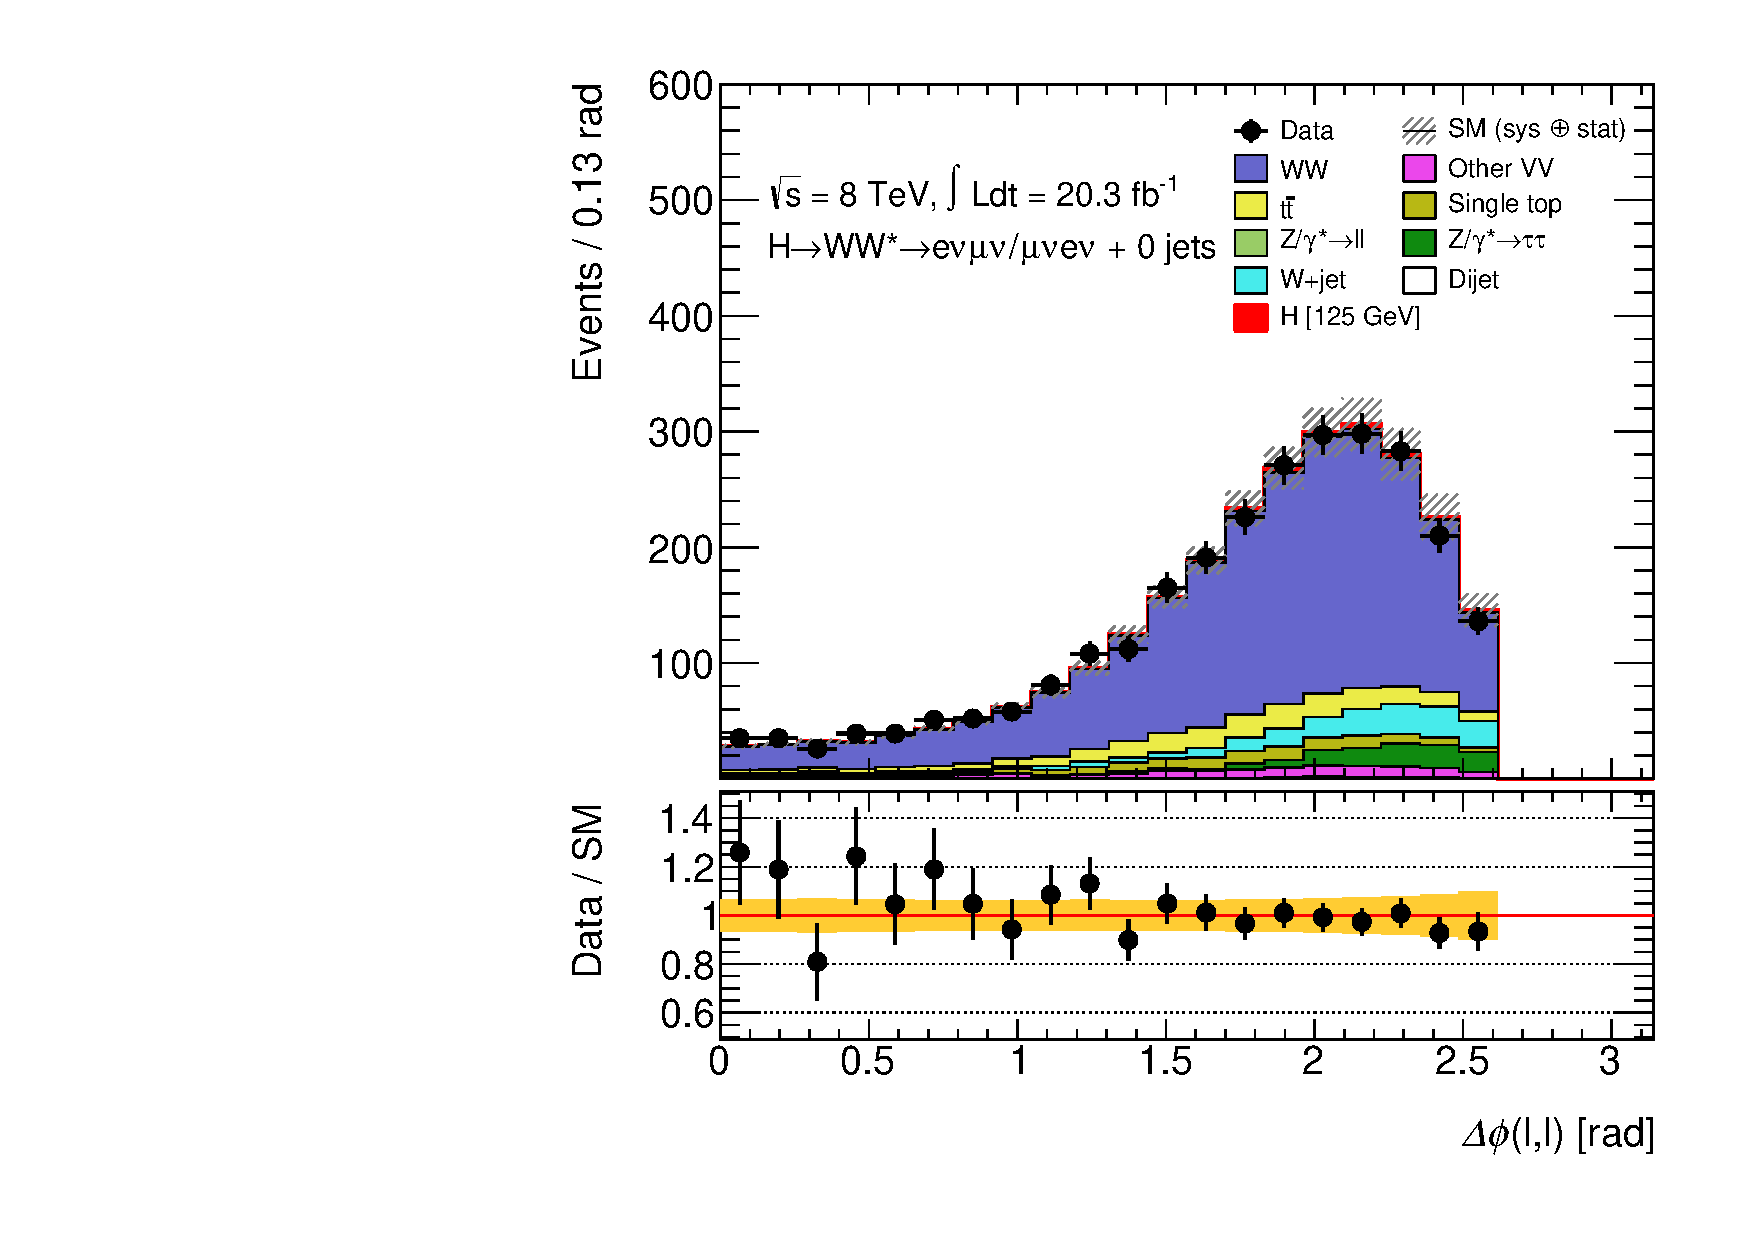
\includegraphics[width=0.495\textwidth]{tex/ww/emme_CutWWControl_0jet_DPhill_mh125_lin}
	\hfill
	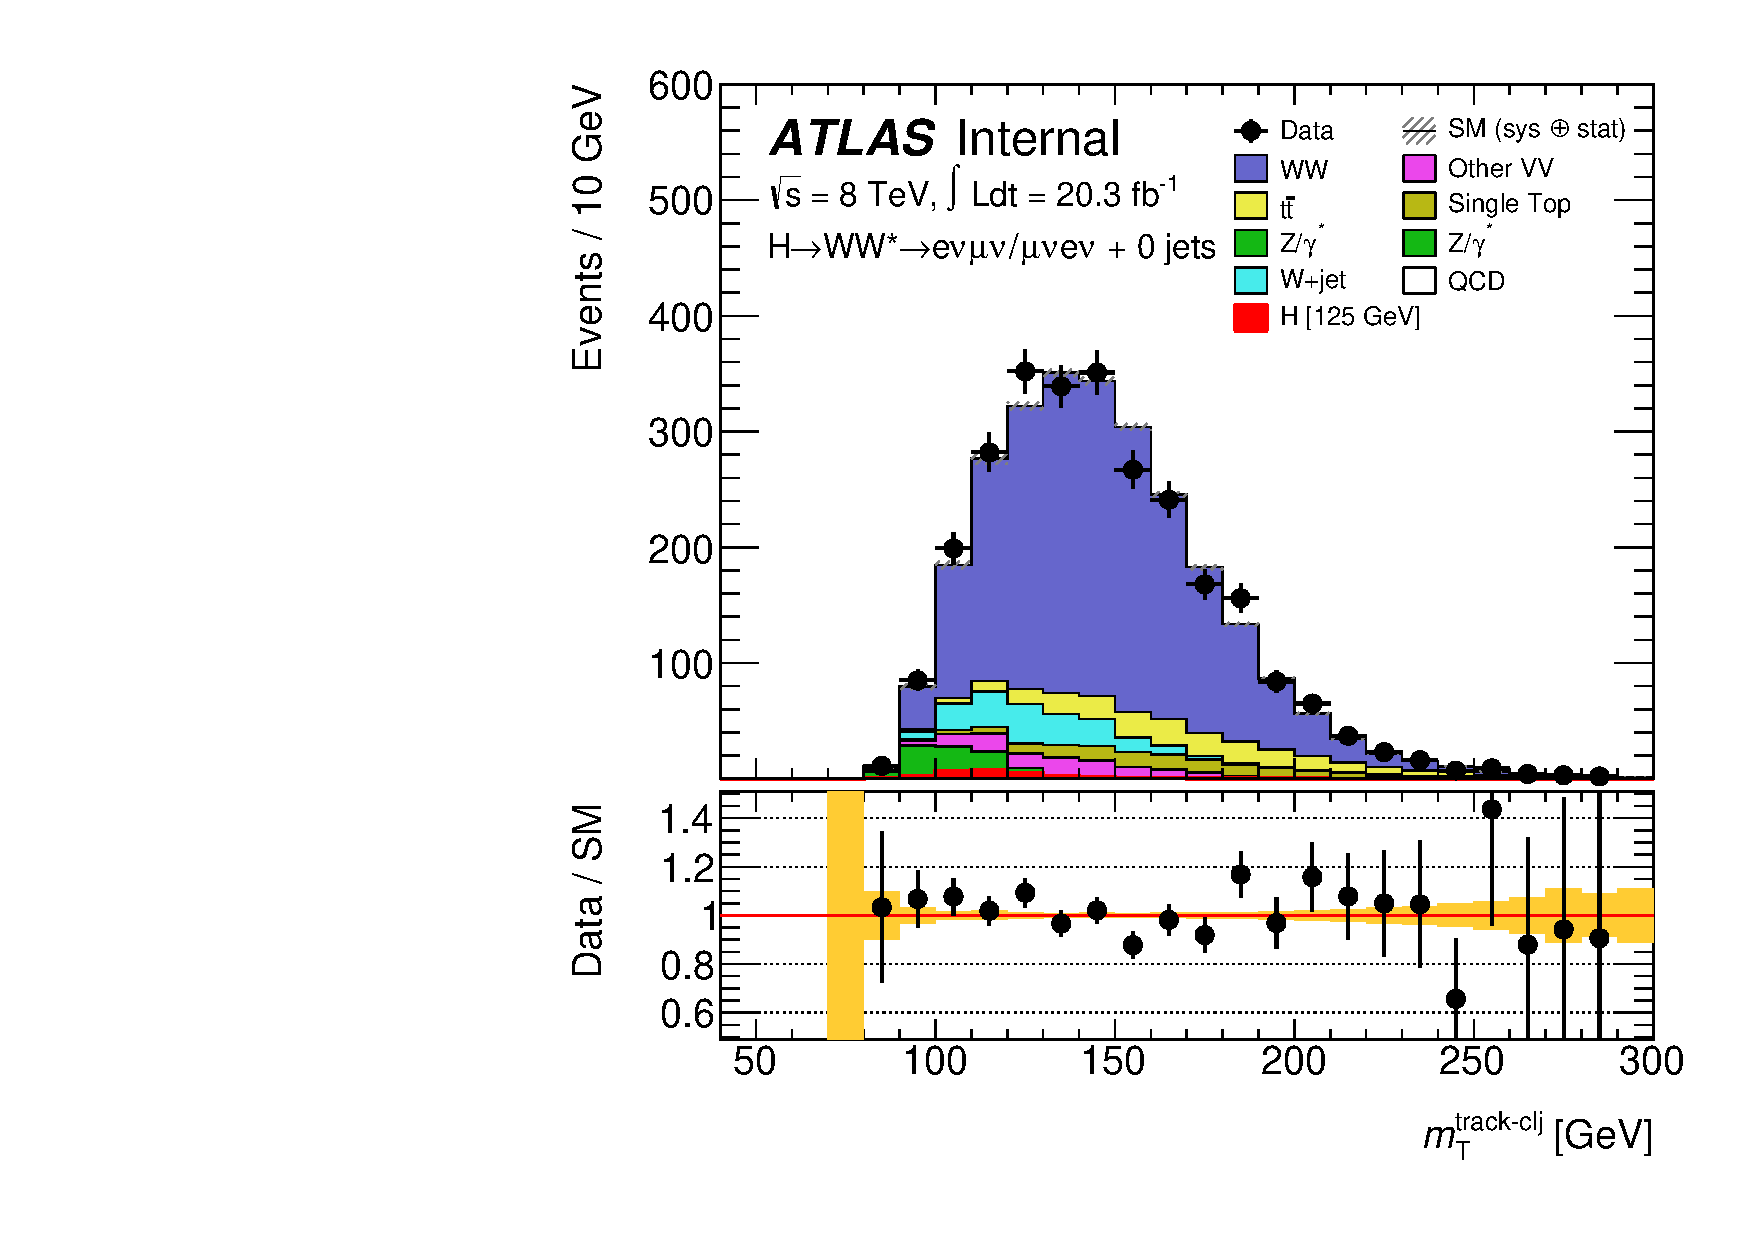
\includegraphics[width=0.495\textwidth]{tex/ww/emme_CutWWControl_0jet_MT_TrackHWW_Clj_mh125_lin}
	\\
	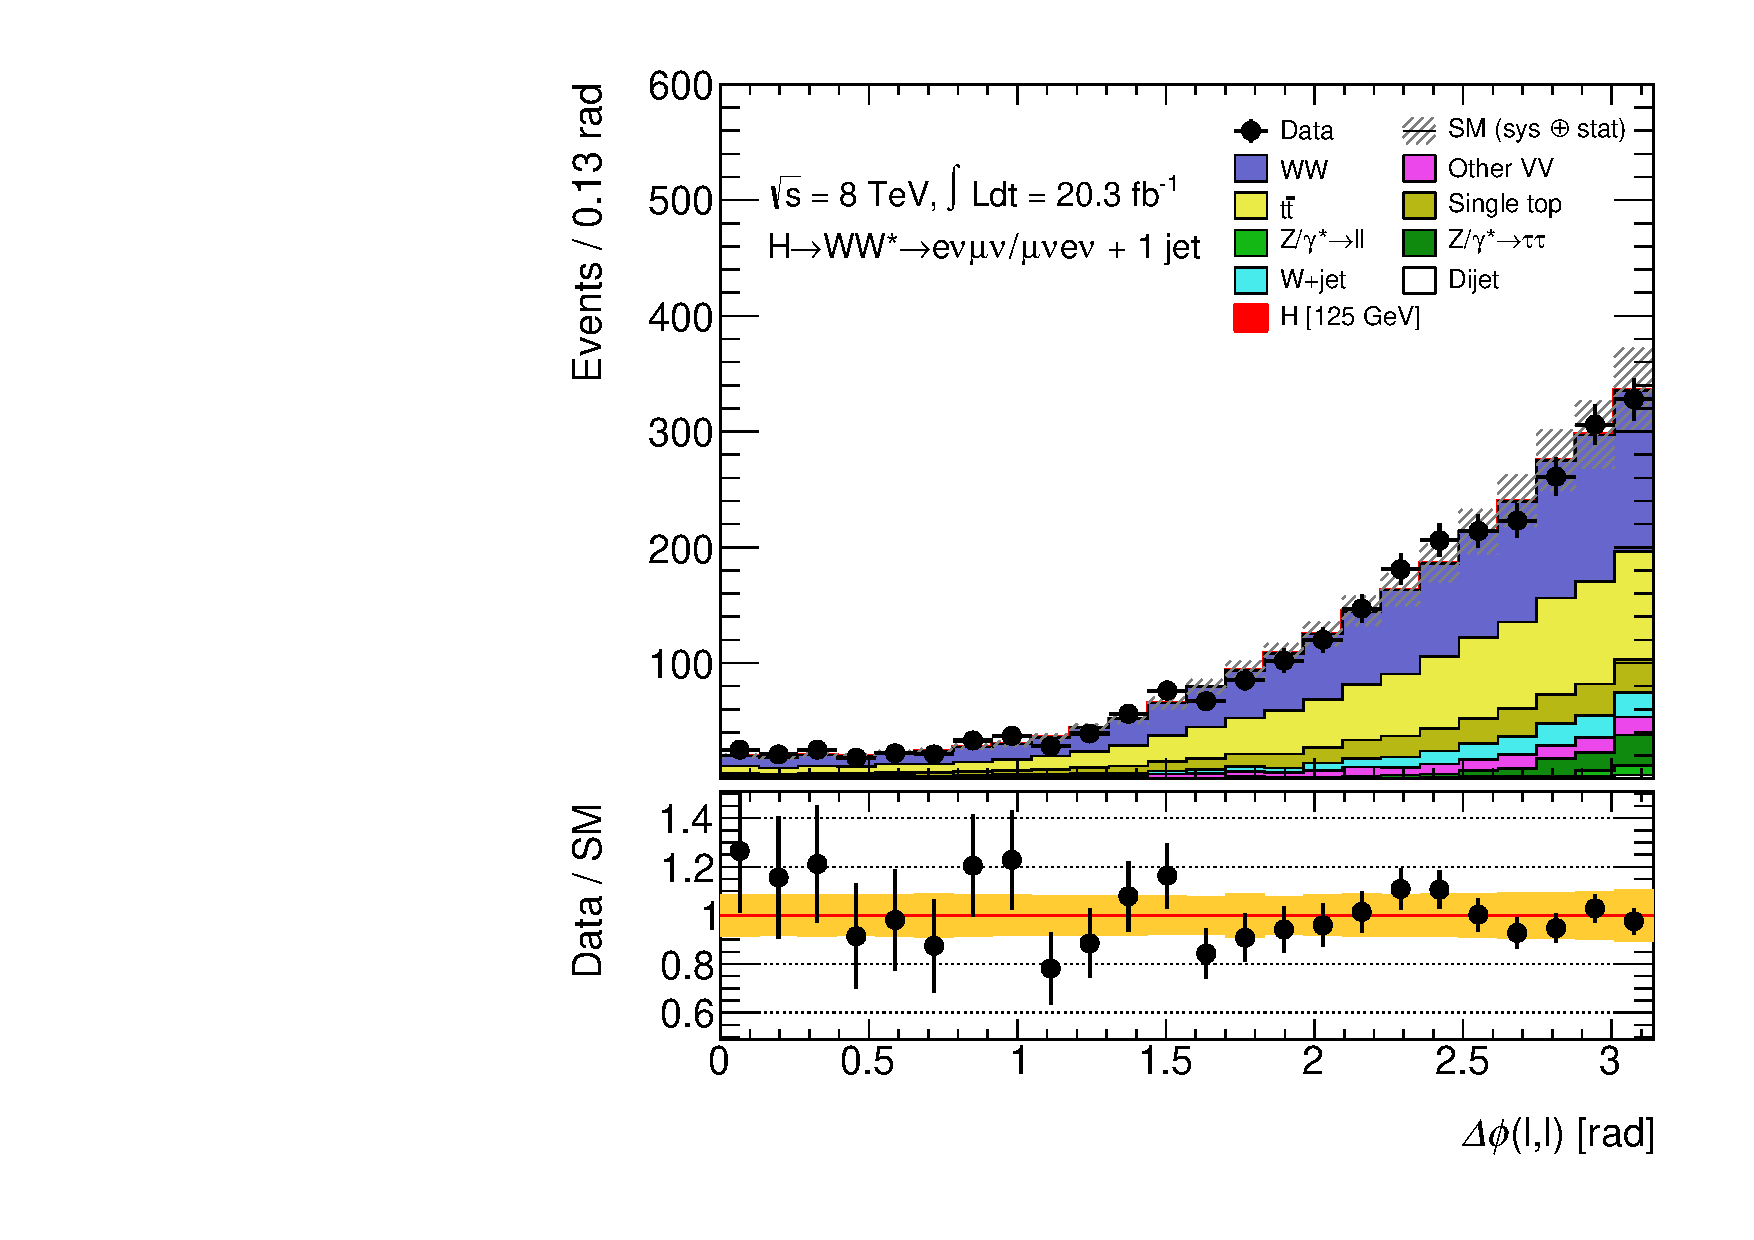
\includegraphics[width=0.495\textwidth]{tex/ww/emme_CutWWControl_1jet_DPhill_mh125_lin}
	\hfill
	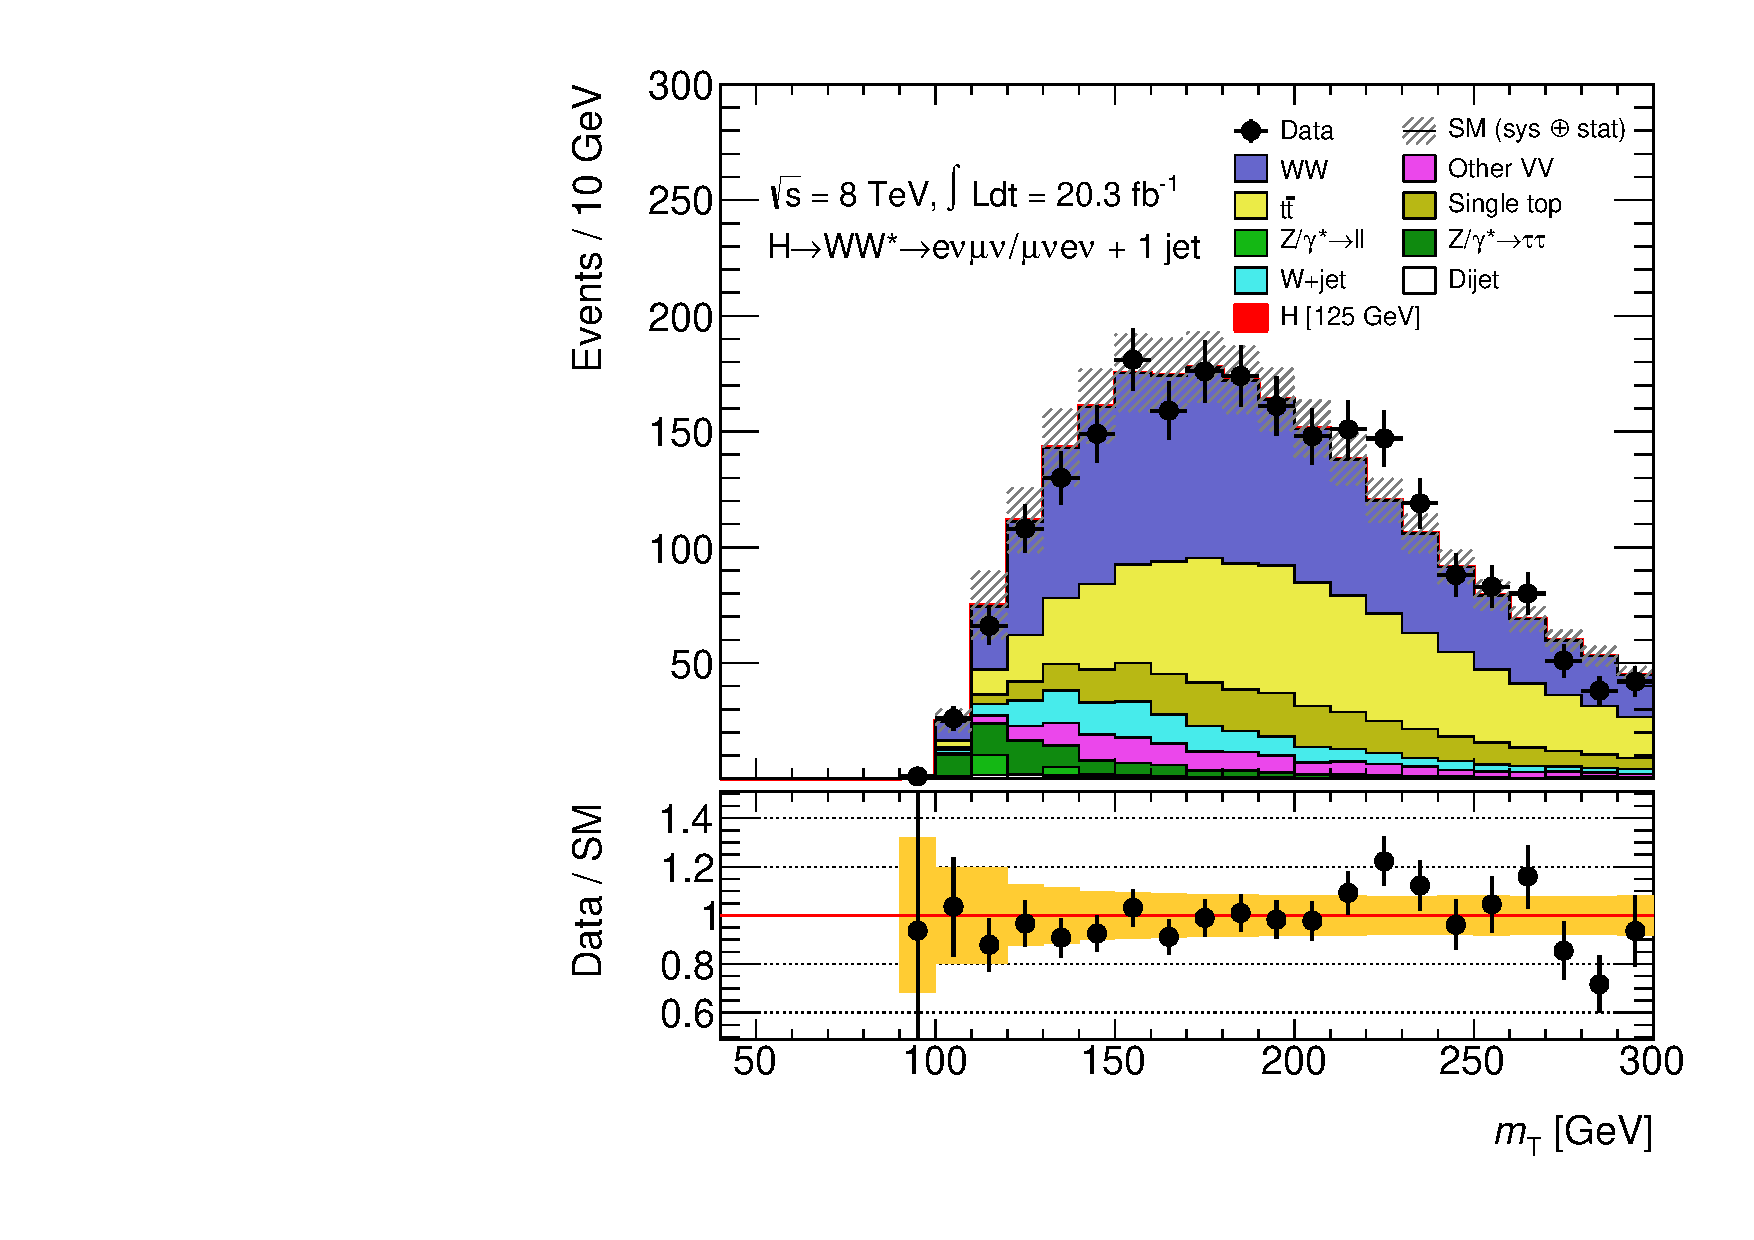
\includegraphics[width=0.495\textwidth]{tex/ww/emme_CutWWControl_1jet_MT_TrackHWW_Clj_mh125_lin}
	\caption{The \dphill (left) and \mt (right) distributions in the \WW control regions 
	of the 0-jet (top) and 1-jet (bottom) bins. Normalisation factors are applied.}
	\label{fig:ww_bkg:cr_plots}
\end{figure}


\subsection{Theoretical uncertainties in $\alpha_{\WW}$}
\label{sec:ww_bkg:alpha}

Theoretical uncertainties in the extrapolation parameters $\alpha_{\WW}$ are evaluated 
at hadron-level (\ie before detector simulation) by changing some aspect of the MC 
modelling and measuring the effect upon each $\alpha_{\WW}$. This is done using NLO \WW 
MC. Uncertainties due to \ggWW diagrams are \about7\%, but have small impact on the 
uncertainty in the measured signal since these diagrams only contribute \about5\% 
(\about7\%) of the \WW background in the 0-jet (1-jet) bin SRs.

The hadron-level event selection criteria used to evaluate these uncertainties are similar 
to the detector-level criteria of the SRs (see \Table~\ref{tab:event_selection}) and CRs 
(see \Table~\ref{tab:ww_cr_sel}), except the \Pbottom-jet veto and \frecoil cuts are omitted.
Hadron-level object definitions are the same as those used for the \WW measurement (see 
\Section~\ref{sec:ww:strategy}), with updated \pt requirements.

Four sources of theoretical uncertainty are considered:
\begin{itemize}[noitemsep,nolistsep]
	\item higher order corrections (QCD and EW),
	\item PDFs,
	\item parton shower, hadronisation and underlying event models,
	\item NLO-PS matching scheme.
\end{itemize}

Uncertainties due to QCD higher order corrections are evaluated via independent variation of 
renormalisation and factorisation scales in the range $\mu_0/2 \leq \mur,\muf 
\leq 2\mu_0$, where $\mu_0 = m_{\HepProcess{\Plepton\Pnu\Plepton'\Pnu'}}$, whilst observing 
the constraint $1/2 \leq \mur/\muf \leq 2$. These are evaluated with \amcatnlo and validated 
with \mcfm. The largest deviation is used as the uncertainty.

Uncertainties due to EW higher order corrections are evaluated by reweighting \powhegbox 
events (based upon the kinematics of the initial state and diboson system) to include NLO EW 
corrections. Such corrections are derived in \Reference~\cite{WW:NLO-EW}.

Uncertainties due to PDFs are evaluated in two ways, which are added in quadrature. 
Predictions with the MSTW 2008 \cite{MSTW} and NNPDF 2.3 \cite{NNPDF} PDF sets are compared 
to those with the CT10 \cite{CTEQ} PDF sets, and the maximum deviation is found. Also, the 
set of PDF eigenvectors corresponding to 90\% CL of the CT10 fit were used to evaluate an 
uncertainty, which was then rescaled to 68\% CL. These are evaluated using \amcatnlo.

Uncertainties due to the PS, hadronisation and UE models are evaluated by 
comparing \powhegbox showered by \pythia{6} (nominal) and by \fherwig. 
Uncertainties due to the NLO-PS matching scheme are evaluated by comparing 
\meps{\powhegbox}{\fherwig} to \meps{\amcatnlo}{\fherwig}.

The $\alpha_{\WW}$ theoretical uncertainties for each SR are shown in 
\Table~\ref{tab:ww_bkg:alpha_unc} (experimental uncertainties are discussed in 
\Chapter~\ref{chap:results}). Although small, they have a large effect in the final fit 
because the \WW background yield is much larger than the signal yield in the SR. 
Extrapolation uncertainties for the VR are also shown. The observed number of events in the 
\WW VR is 10\% higher than expected, corresponding to a $0.65\sigma$ deviation when 
statistical and systematic uncertainties are considered. This agreement supports the 
extrapolation uncertainties assigned to the SRs.

\begin{table}[t]
	\centering
	\begin{tabular}{ccc|cccccc}
		\toprule
		& \mll & \ptsubleadlep & \multicolumn{2}{c}{Scale} & \multicolumn{2}{c}{PDF} & \multirow{2}{*}{PS/UE} & \multirow{2}{*}{NLO-PS} \\
		& (\GeV) & (\GeV) & QCD & EW & collab. & 68\% CL & & \\
		\midrule
		\multicolumn{9}{c}{\eech/\mmch channels} \\
		\midrule
		0-jet & 12--55 & $>10$ & 0.8\% & $+0.1\%$ & 0.5\% & 1.0\% & $-1.2\%$ & $+2.4\%$ \\
		1-jet & 12--55 & $>10$ & 0.8\% & $-2.1\%$ & 0.5\% & 0.7\% & $-2.3\%$ & $+3.8\%$ \\
		\midrule
		\multicolumn{9}{c}{\emch/\mech channels} \\
		\midrule
		\multirow{6}{*}{0-jet}
		& \multirow{3}{*}{10--30}
	    &  10--15 & 0.7\% & $+1.2\%$ & 0.9\% & 0.2\% & $+2.2\%$ & $+0.4\%$ \\
		&& 15--20 & 1.2\% & $+0.7\%$ & 0.8\% & 0.2\% & $+1.7\%$ & $+0.9\%$ \\
		&&  $>20$ & 0.7\% & $-0.3\%$ & 0.5\% & 0.3\% & $-1.9\%$ & $+3.1\%$ \\
		\cmidrule(lr){2-9}
		& \multirow{3}{*}{30--55}
		&  10--15 & 0.7\% & $+0.8\%$ & 0.8\% & 0.1\% & $+1.5\%$ & $+0.5\%$ \\
		&& 15--20 & 0.8\% & $+0.5\%$ & 0.7\% & 0.2\% & $+1.0\%$ & $+1.0\%$ \\
		&&  $>20$ & 0.8\% & $-0.4\%$ & 0.4\% & 0.5\% & $-2.4\%$ & $+3.9\%$ \\
		\cmidrule(lr){1-9}
		\multirow{6}{*}{1-jet}
		& \multirow{3}{*}{10--30}
	    &  10--15 & 3.1\% & $-0.9\%$ & 0.5\% & 0.1\% & $-2.4\%$ & $-3.4\%$ \\
		&& 15--20 & 1.6\% & $-1.5\%$ & 0.5\% & 0.1\% & $-3.0\%$ & $+0.7\%$ \\
		&&  $>20$ & 1.0\% & $-2.8\%$ & 0.6\% & 0.2\% & $-3.6\%$ & $+5.3\%$ \\
		\cmidrule(lr){2-9}
		& \multirow{3}{*}{30--55}
		&  10--15 & 3.2\% & $-0.9\%$ & 0.5\% & 0.1\% & $-2.0\%$ & $+1.9\%$ \\
		&& 15--20 & 1.5\% & $-1.6\%$ & 0.4\% & 0.1\% & $-3.0\%$ & $+2.4\%$ \\
		&&  $>20$ & 1.3\% & $-2.7\%$ & 0.5\% & 0.4\% & $-3.1\%$ & $+5.6\%$ \\
		\midrule
		\multicolumn{9}{c}{Validation region (\emch/\mech channels)} \\
		\midrule
		0-jet & $>110$ & $>15$ & 0.6\% & $+1.6\%$ & 0.6\% & 2.0\% & $+4.3\%$ & $-5.1\%$ \\
		\bottomrule
	\end{tabular}
	\caption{Theoretical uncertainties in the \WW extrapolation parameter $\alpha_{\WW}$ 
	for each signal region used in the fitting procedure, and also for the validation 
	region.}
	\label{tab:ww_bkg:alpha_unc}
\end{table}



\subsection{\mt shape modelling}
\label{sec:ww_bkg:mt}

Theoretical uncertainties in the shape of the \mt distribution are also investigated, 
as they affect the fit. Uncertainties due to scale, PS/UE and NLO-PS choices are 
considered within each signal region separately, using the methods described above.

Each uncertainty is parametrised by fitting the ratio of the \mt shapes, and then 
symmetrising the fit to produce ``up'' and ``down'' variations. The \mt distributions are 
normalised to unit integral in order to probe only shape uncertainties. A linear 
fit is used in the central \mt region, and a constant is used in the low-\mt and 
high-\mt tails of the distribution where statistical fluctuations dominate.

These fits allow the hadron-level \mt distribution of the \WW background to be reweighted 
to the ``up'' and ``down'' variations. In this way, the \mt shape uncertainty is treated 
as a nuisance parameter in the \HWW fitting procedure (see \Chapter~\ref{chap:results}). 
The uncertainties for the split signal regions of the \emch/\mech channels are displayed in 
Figures~\ref{fig:ww_bkg:mTshape_0j} and \ref{fig:ww_bkg:mTshape_1j} for the 0-jet and 1-jet 
bins, respectively.

\begin{figure}[p]
	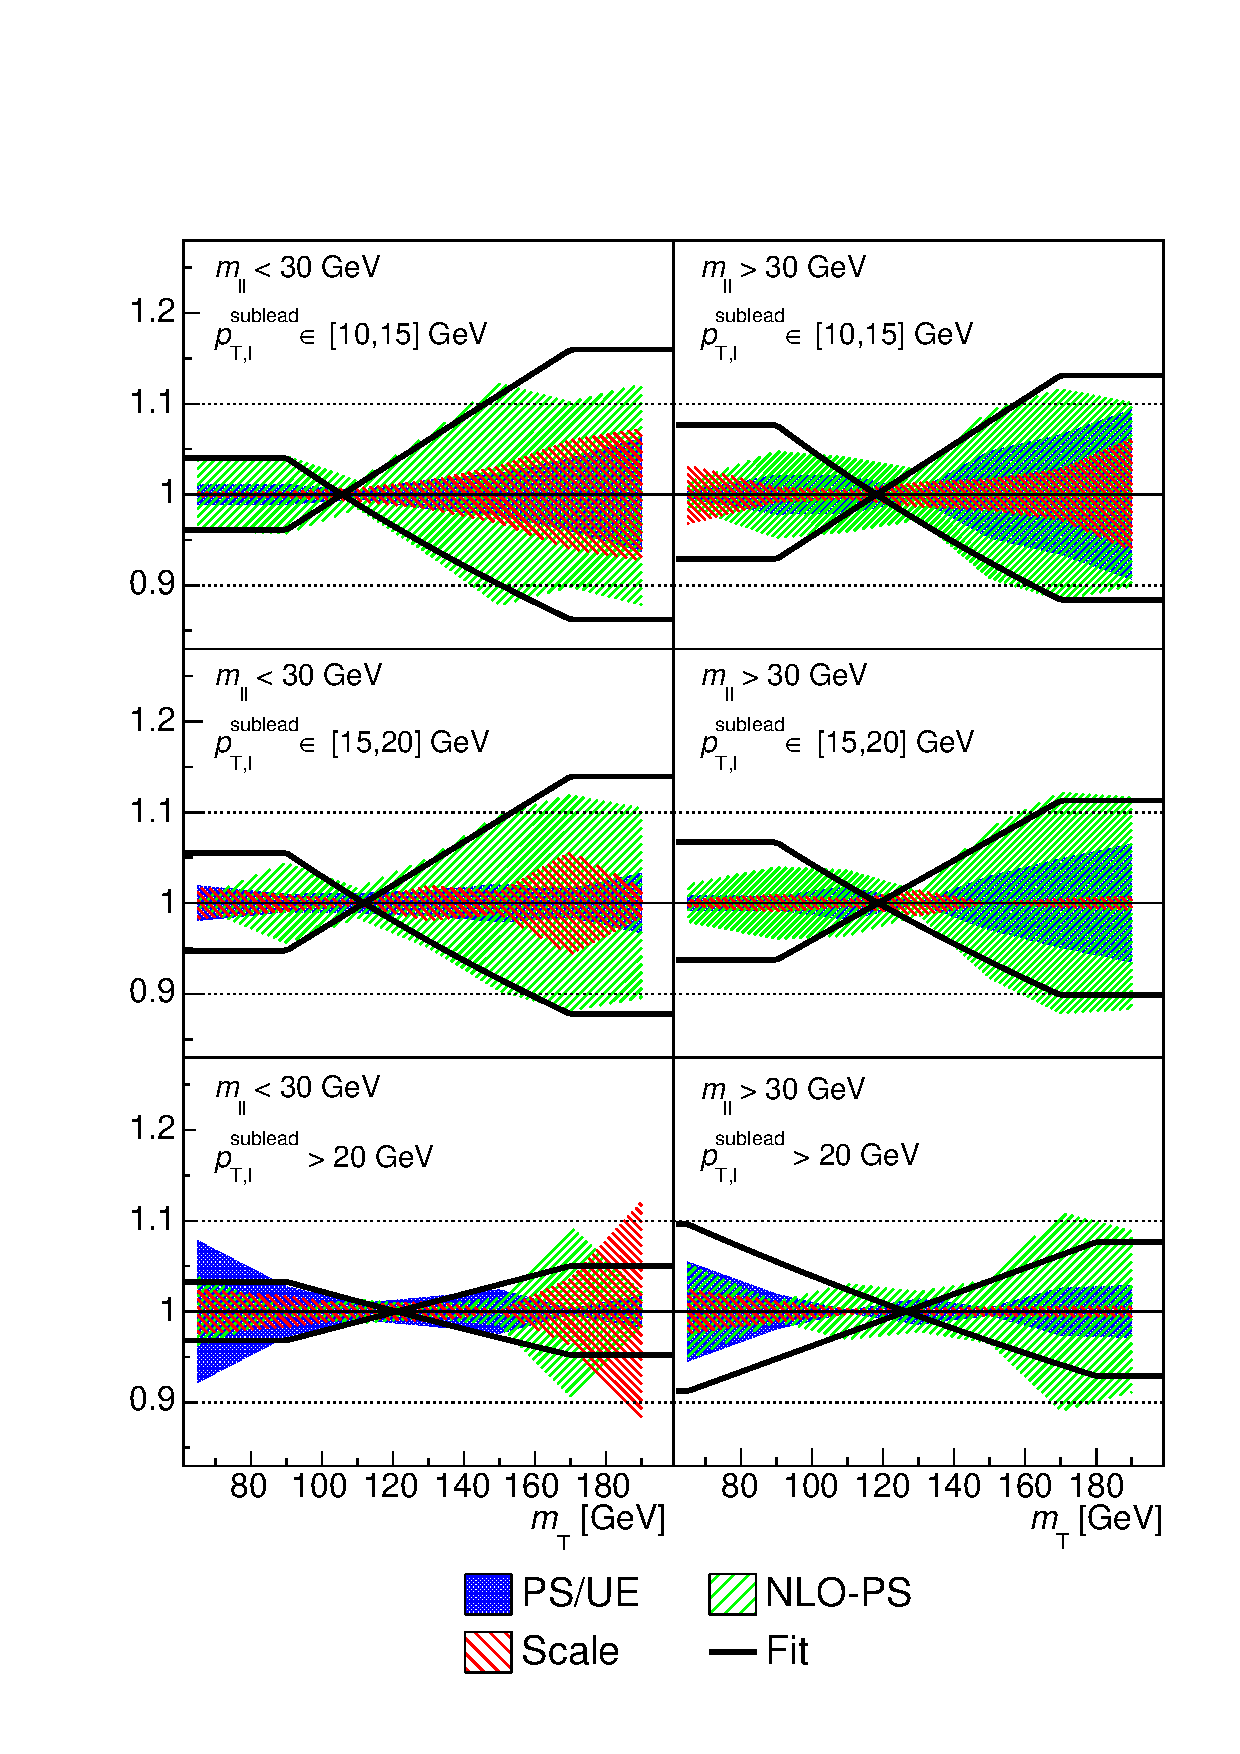
\includegraphics[width=\hugefigwidth]{custom_images/mT-shapes/ww_df_0j}
	\caption{\WW \mt shape systematic uncertainties in each 0-jet signal region for the 
	\emch/\mech channels. The fit shown is the sum in quadrature of the three individual 
	fits, and successfully envelopes the uncertainty sources.}
	\label{fig:ww_bkg:mTshape_0j}
\end{figure}

\begin{figure}[p]
	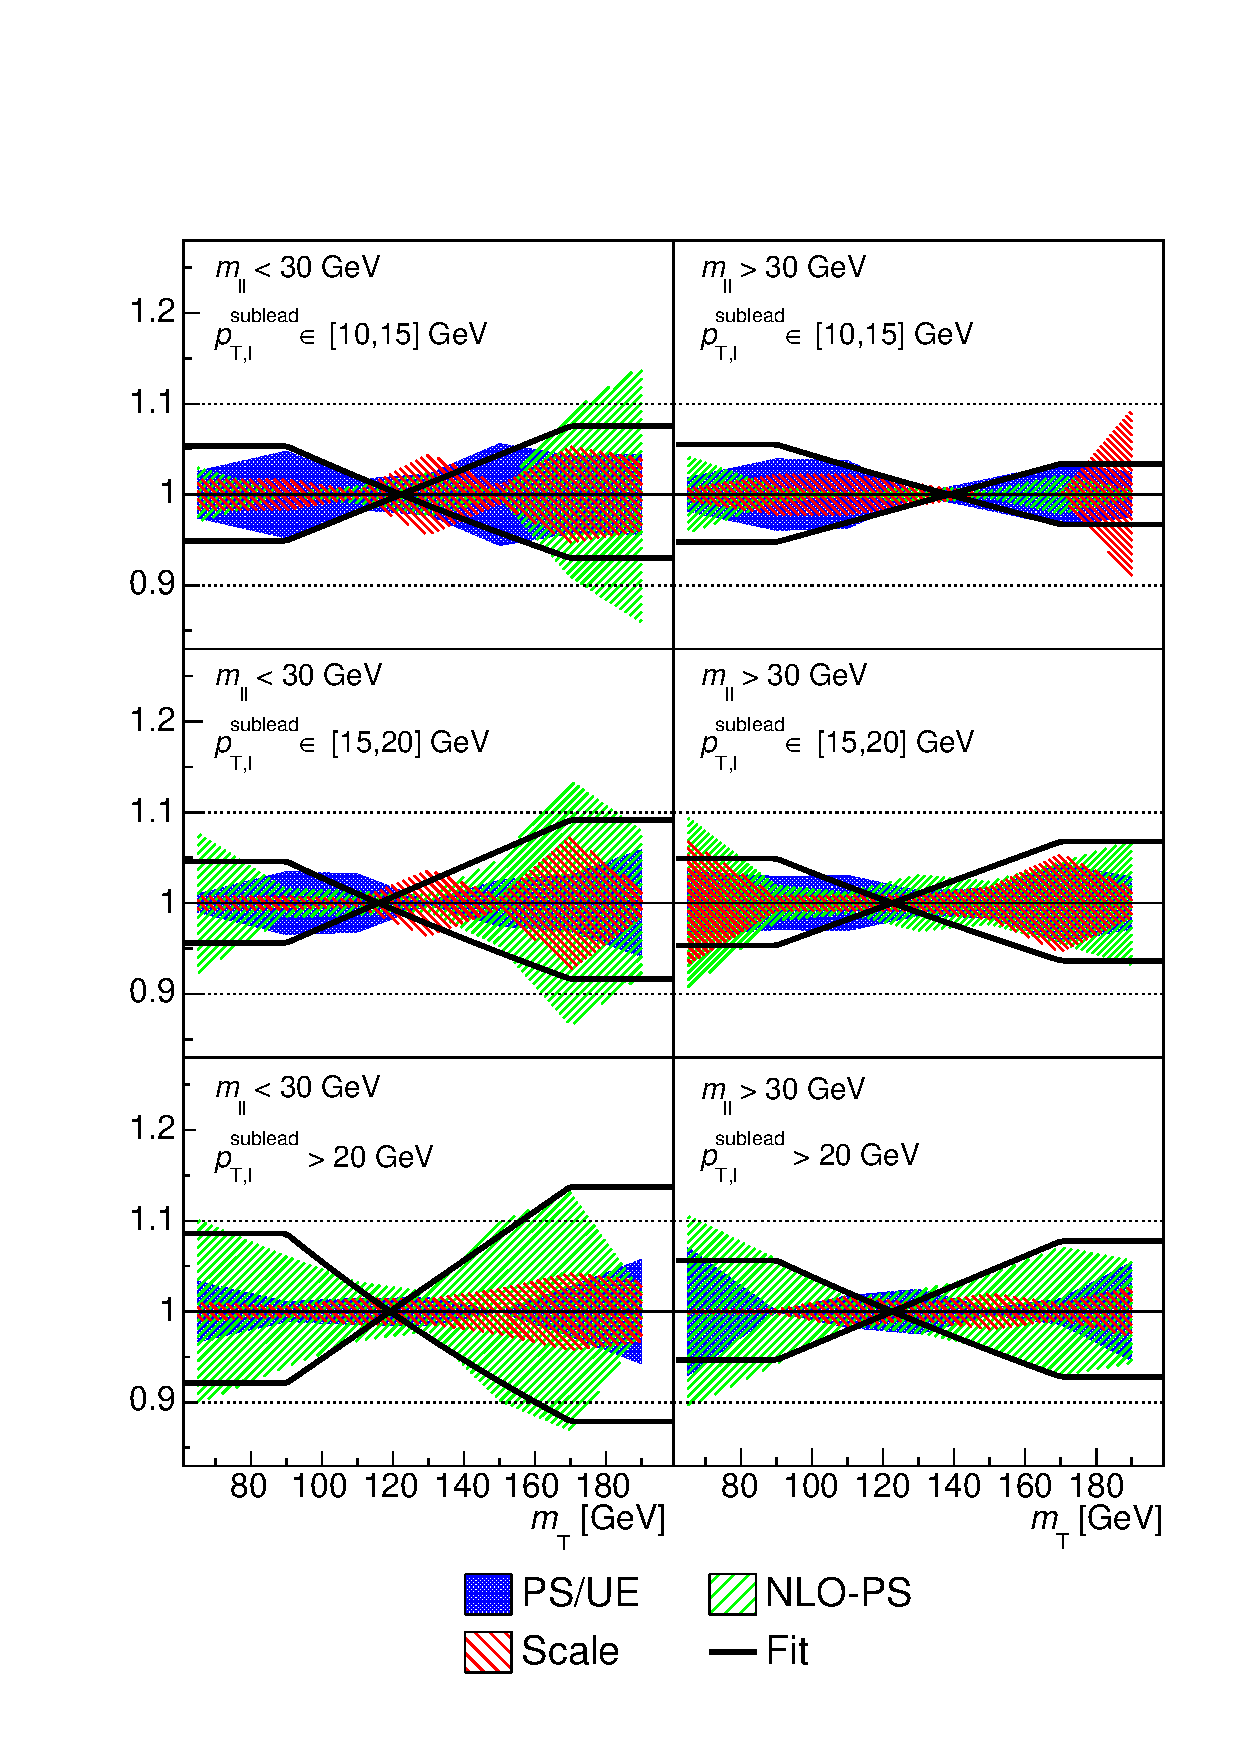
\includegraphics[width=\hugefigwidth]{custom_images/mT-shapes/ww_df_1j}
	\caption{\WW \mt shape systematic uncertainties in each 1-jet signal region for the 
	\emch/\mech channels. The fit shown is the sum in quadrature of the three individual 
	fits, and successfully envelopes the uncertainty sources.}
	\label{fig:ww_bkg:mTshape_1j}
\end{figure}



\subsection{\WW background in the \twojet bin}
\label{sec:ww_bkg:2j}

\powhegbox relies upon the parton shower to produce the second emission; consequently events 
with two or more hard jets are likely to be poorly modelled. For this reason, \sherpa is 
used to describe the \WW background in the \twojet bin, including up to three partons in the 
matrix element using LO ME-PS merging (see \Section~\ref{sec:mc:merging}).

Two kinds of diagrams can be identified for the \WW~+~2~jets process: EW production (zero 
QCD vertices at LO) and QCD production (two QCD vertices at LO), where VBF \WW production is 
included in the former. The two production types are simulated separately by \sherpa, and 
this causes their interference to be neglected. Interference with VBF Higgs boson production 
is also neglected. The effect of each interference is investigated and treated as a 
systematic uncertainty.

Uncertainties due to the choice of \mur and \muf scale are considered, and also a modelling 
uncertainty is evaluated by comparing the \sherpa yield to that of 
\meps{\madgraph}{\pythia{6}}. The uncertainty in QCD \WW~+~2~jets production is \about20\%, 
and the uncertainty in EW \WW~+~2~jets production is \about10\%.

